\documentclass[11pt]{article}
\usepackage{ctex}

\usepackage[left=1.25in,right=1.25in,top=1in,bottom=1in]{geometry}
\usepackage{graphicx}
\graphicspath{{figures/}}

\usepackage{fontspec}
\usepackage{amsthm,amsmath,amssymb,mathrsfs}

\begin{document}
	\title{Some imformation about article}
	
	\maketitle
	
	\newpage
	\tableofcontents
	\newpage

\section{Simple Baselines for Human Estimation and Tracking}
\subsection{Introduction}

Algorithm and system complexity increase.The paper provides simple and effective baseline methods.Many vision tasks are significantly advanced by deep learning.

There are two state-of-the-art network architectures for pose estimation:
1.one stage in Hourglass.
2.CPN(Cascaded Pyramid Network)

The main task of pose estimation is 'how high resolution feature maps are generated'.In other words 'Obtaining high resolution feature maps is crucial,but no matter how.

The steps of Multi-person pose tracking in videos:
1.estimate human poses in frames.
2.track these human pose by assigning a unique ID to them across frames.

Pose tracking is the task of estimating multi-person human poses in videos and assigning unique instance IDs for each keypoint across frames.

We will expand the box where propagate joint location 15\% in experiments.We could have boxes propagated from previous frames where people have been detected correctly.We can track result in previous frames.


\subsubsection{The past reasult in some dataset}

MPII benchmsrk starte from about 80\% PCKH@0.5 to more than 90\%.The leading methods on MPII benchmark have considered many details in different wats but minor difference in accuracy.

COCO human pose benchmark is even faster, the mAP metric is increased from 60.5 to 72.1

\subsection{Network}

Resnet is the most common backbone network for image feature extraction.Resnet is the simplest way to estimate heat maps from deep and low resolution feature maps.(mAP of 73.7 on COCO testdev split)

The network of this paper is a backbone network(ResNet) with a few deconvolutional layers(C5).C5 uses the batch normalization and Relu activation.We adopt this structure because it is arguably the simplest to generate heatmaps from deep and low resolution features and also adopted in the Mask R-CNN

The Greedy matching algorithm is about how to repeat the ID or assign a new ID number.(Mask RCNN and greedy bipartite matching algorithm)

\begin{figure}[h]
	\centering
	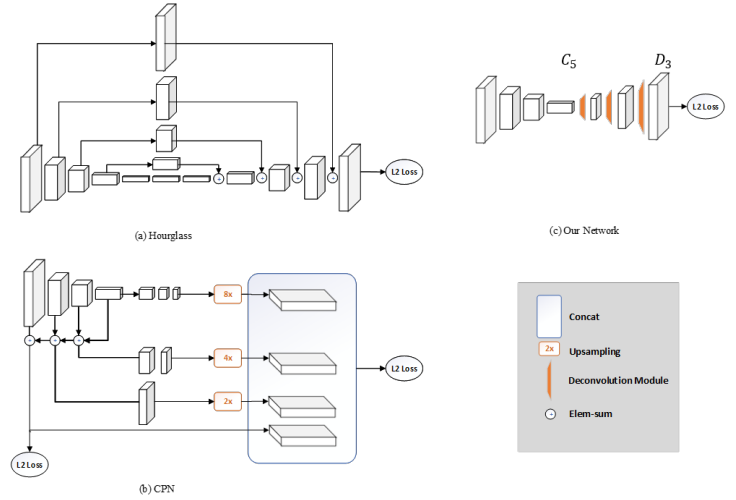
\includegraphics[scale = 0.5]{1}
\end{figure}

Mean Squared Error(MSE) is used as the loss between the presicted heatmaps and targeted heatmaps.

Some detector for single image level or maybe videos (Faster-RCNN,R-FCN)

The flow-based inference algorithm for video human pose tracking

The first problem is pose estimation problem(mainly use a bounding box Non-Maximum Suppression(NMS))
The second problem is tracking problem(mainly the Q used to capture previous multi frames' linking relationship,the Q's length indicates how many previous frames considered when performing matching)

INPUT:

video frames(A), Q = [](Q's max capacity LQ)

Process:

1.person detection network to get person (B)

2.meantime video frame(B)and frame that get person(A) get into human pose estimation network can get the first frame(C)

3.initialize the id for the first frame(C)

4.append id and the first frame(C) into Q

5.get into the loop to deal with video frames after the first frame

LOOP(k = 1 to inf):

1.person detection network to get person

2.put the before human pose estimation network's reasult(k-1) and flow field frame k-1 to frame k to generate boxes by joint propagating

3.use NMS(Non-Maximum Suppression) to unify detection boxes and flow boxes

4.use NMS'result and the k frame into human pose estimation network to get(J)

5.put G and Q to get into funtion for similarity matrix to get similarily matrix(M)

6.put M and J into function for assigning instance id to get the frame unique id(P)

7.append the P to the Q(update the Q)

\begin{figure}[h]
	\centering
	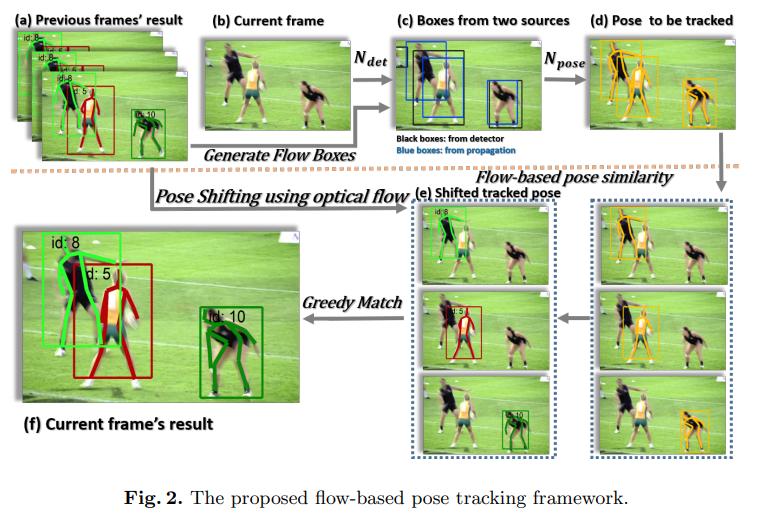
\includegraphics[scale = 0.5]{2}
\end{figure}

\subsection{Conclusions and Contributions}

We present simple and strong baseline for pose estimation and tracking.The contribution of the work are soild baselines for the field(in other words,after this paper the results of other reaserch must do better than the reasult in this paper)

1.Two different kind of human boxes(one is a human detector, other is boxes generated from previous frames using optical flow)

2.Using a metric similar with greedy matching algorithm
\subsection{The direction after this paper}

"Simultaneous pose dectation and tracking in wild" or the pose tracking(Using the greedy matching method) 
\section{LightTrack: A Generic Framework for Online Top-Down Human Pose Tracking}
\subsection{Abstract}
The proposed framework is designed to be generic for top-down pose tracking and is faster than existing online and offline methods.

Single-person Pose Tracking(SPT) and Visual Object Tracking(VOT) are incorporated into one unified functioning entity,replaced single-person pose estimation module.

Our framework unifies single-person pose tracking with multi-person identity association.Bridging keypoint tracking with object tracking.

Siamese Graph Convolution Network(SGCN) for human pose matching as a Re-ID module(using a graphical representation of human joints for matching ) in our pose tracking system.

The skeletonbased representation effectively captures human pose similarity and is computationally inexpensive.

It is robust to sudden camera shift that introduces human drifting.

To the best of our knowledge, this is the first paper to propose an online human pose tracking framework in a top-down fashion.

The proposed framework is general enough to fit other pose estimators and candidate matching mechanisms.

Our method outputforms other online methods while maintaining a much higher frame rate, and is very competitive with our offline state-of-the-art.
\subsection{Introduction}
Accurate estimation of human keypoint-trajectories is useful for human action recognition, human interaction understanding, motion capture and animation.

More emphasis has been put on the Multi-Object Tracking Accuracy(MOTA) criterion compared to the Frame Per Second(FPS) criterion.

In this paper,we propose anovel effective light-weight framework for pose tracking.

We track each human pose by recursively updating the bounding box and its corresponding pose in an explicit manner.

The bounding box region of a target is inferred from the explicit features(the human keypoints)

The advantages of using pose as explicit features include:

(1).The explicit features have very strong and stable relationship with the bounding box position.

(2).Tracking requires human keypoints,taking advantage of the predicted keypoints is efficient in tracking the ROI region.

(3).

Most exising methods are offline hence lacking the potential to be real-time.
\subsection{Related Work}
\subsubsection{Human Pose Estimation and Tracking(HPE)}

Multi-person human pose estimation is more realistic and challenging.

Existing methods can be classified into top-down and bottom-up approaches.

The top-down approaches rely on the detection module to obtain human candidates and then applying single-person pose estimation to locate human keypoints.

The advantage of top-down approaches is their capability in disassembling the task into multiple comparatively easier tasks(object detection and single-person pose estimation) 

The bottom-up methods detect human keypoints from all potential candidates and then assemble these keypoints into human limbs for each individual based on various data association techniques.

The advantage of bottom-up approaches is thire excellent trade-off between estimation accuracy and computational cost because the cost is nearly invariant to the number of human candidate in the image.


\subsection{Conclutions and Contributions}

Our method outperforms other online methods while maintaining a higher frame rate, and is very competitive with our offline state-of-the-art

The proposed framework is general enough to fit other pose estimators and candidate matching mechanisms.

\section{PoseTrack A Benchmark for Human Pose Estimation and Tracking}

\subsection{Abstract}

Exising systems for video-based pose estimation and tracking struggle to perform well on realistic videos with multiple people and often fail to output body-pose trajectories consistent over time.

To address this shortcoming this paper introduces PoseTrack which is a new large-scale benchmark for video-based human pose estimation and articulated tracking.

Our new benchmark encompasses three tasks focusing on i)single-frame multi-person pose estimation, ii)multi-person pose estimation in videos, iii)multi-person articulated tracking.

new dataset,LSP,LSP Extended,MPII Human Pose(Single Person),MS COCO Keypoint Challenge,else in table 1.

\subsection{Introduction}

Importantly, these benchmark datasets not only have provided extensive training sts required for training of deep learning based approaches, but also established detailed metrics for direct and fair performance comparison across numerous competing approaches.

Significant progress of single frame based multiperson pose estimation.It's still problem about articulated multiperson body joint tracking in monocular video.

In the work,we aim to fill this gap by establishing a new large-scale, high-quality benchmark for video-based multi-person pose estimation and articulated tracking. 

Three related tasks focuse on 1.single-frame multi-person pose estimation,2.multi-person pose estimation in video,3.multi-person articulated tracking.

\subsection{Data Annotation}

We annotated the selected video sequences with person locations, identities, body pose and ignore regions.

The annotations are about four steps:
1.we labele ignore regions to exclude crowds and people for which pose can not be relibly determined due to poor visibility.
2.the head bounding boxes for each person across the videos are annotated and a track ID is assigned to each person.
3.assign a unique track ID to each person appearing in the video until the person moves out of the camera field-of-view
4.maintain track ID between shots and same person might get different track ID if it reappears in another shot

Annotation strategy:for each sequence in our benchmark we annotate the 30 frames in the middle of the sequence.In addition, we annotate validation and test sequences with a step of four frames.(aim to evaluate both smoothness of body joint tracks as well as ability to track body joints over longer number of frames)

\subsection{Challenges}

The benchmark consists of the following challenges:

Single-frame pose estimation:this task is similar to the ones covered by existing datasets like MPII Pose and MSCOCO Keypoints.

Pose estimation in videos:the evaluation of this challenge is performed on single frames,but the data will also include video frames before and after the annotated ones.

Pose tracking:this task requires to provide temporally consistent poses for all people visible in the videos.
\subsection{Experimental Setup}

In order to evaluate whether a body part is predicted correctly, we use the PCKh(head-normalized probability of correct keypoint) metric, which considers a body joint to be correctly localized if the predicted location of the joint is within a certain threshold from the true location.

Due to large scale variation of people across videos and even within a frame, this threshold needs to be selected adaptively based on the person's size

Two sets of evaluation metrics:one use for evalusting multi-person pose estimation,one from the multi-target tracking literature to evaluate multi-person pose tracking.

We ignore all person detections that overlap with the ignore regions.

Multi-person pose estimation:we use mean Average Precision(mAP) to measure frame-wise multi-person pose accuracy.(way:we propose not to use any ground-truth information during testing and evaluate the predictions without rescaling or selecting a specific group of perple for evaluation)

Evaluate multi-person pose estimation requires that the location of a group od persons and their rough scale is known during evaluation,but this information is never available in realistic scenarios,particularly for videos.

Articulated multi-person pose tracking:we use MOT(Multiple Object Tracking)metrics and  apple them independently to each of the body joints

The way to get MOT metrics(require predicted body poses with track IDs):1.Compute distances between predicted and ground-truth locations for each frame, for each body joint class. 2.Match predicted and ground-truth locations by a global matching procedure that minimizes the total assignment distance. 3.Compute MOTA(Multiple Object Tracker Accuracy),MOTP(Multiple Object Tracker Precision),Precision and Recall metrics


\subsection{The State of Art}

Articulated pose tracking in unconstrained videos is a relatively new topic in compuer vision research.

We processed in two ways to analyze the performance of the state of the art on our new dataset.

First, we propose two baseline methods based on the state-of-the-art approaches.We modify these methods to make them applicable on our proposed dataset.

Second,in order to broaden the scope of our evaluation we organized PoseTrack Challenge in conjunction with ICCV'17 our dataset by establishing an online evaluation server and inviting submissions from the research community.

\section{Pose Recognition with Cascade Transformers}

\subsection{Abstract}

We present a regression-based pose recognition method using cascade Transformers.We utilize the encoder-decoder structure in the Transformers to perform regression-based person and keypoint detection that is general-purpose and requires less heuristic design compared with the existing approaches.

One way to categorize the existing approaches in this domain is to separate them into 1.heatmap-based 2.regression-based.

Heatmap-based methods can achieve higher accuracy but are subject to various heuristic desighs(not end-to-end mostly).

Regression-based methods have less intermediate non-differentiable steps but lower accuracy.

We demonstrate the keypoint hypothesis(query) refinement process across different self-attention layers to reveal the recursive self-attention mechanism in Transformers. 

\subsection{Introduction}

Pose recognition is a challenging problem that remains unsolved.The difficulty lies in various aspects such as large pose/shape variation,inter-person and self occlusion,large appearance variation,and background clutter.

The task of pose recognition is to localize the human keypoint(17 in the experiments) for the individual persons in two ways.

1.Top-down process:persons are detected first,followed by keypoint detection from the detected image region/patch.

2.Bottom-up process:human keypoints are detected directly from the image without an explicit object detection stage.

3.Heatmap or Regression:heatmap-based methods are adopted when the accuracy is the priority whereas regression-based approaches can be considered as a convenient plug-and-play module.

Heatmap approaches perform dense keypoint detection followed by subsequent processes for clustering and grouping;they deliver strong performance but are also subject to many heuristic designs that are mostly not end-to-end learnable.

Regression perform regression for the keypoints directly which have less intermediate stages and specifications.

DARK presents Taylor-expansion based coordinate decoding and unbiased sub-pixel centered coordinate encoding.

UDP even discovered a considerable accuracy decrease when using one-pixel flip shift in heatmap-based paradigms.

For general-purpose regression methods, we aim at removing unnecessary designs by making the training objective and target output direct and transparent.Coordinates should be output direct and loss be calculated with predictions and ground truth coordinates straightforward.

We present a top-down regression-based 2D human pose recognition method using cascade Transformers consisting of a person detection Transformer and a keypoint detection Transformer.

Two alternatives in Pose Recognition with TRansformer(PRTR):1.a two-stage process 2.a sequential process with the two transformers(end-to-end).

We apply multi-scale features in the keypoint detection Transformer.

\subsection{Contributions}

1.We propose a regression-based human pose recognition method(PRTR) by buliding cascade Transformers,based on a general-purpose object detector,end-to-end object detection Transformer(DETR).

Tokenized representation in Transformers with layers of self-attention to capture the joint spatial and appearance modeling for the keypoints.

2.Two types of descade Transformers:1.two-stage process;2.sequential use spatial Transformer network(STN)

3.We visualize the distribution of keypoint queries in various aspects to unfold the internal process of the Transformer for the gradual refinement of日 the detection.

As far as we know, we are the first to visualize the dynamic decoding process in Transformer decoder, which brings significant insights to future Transformer designs.But there are limited visualization works compared with those done on language application.
\subsection{Related Work}

HRNet family model(advance for 2D human pose recogniton/estimation) is itself about a new convolutional neural network(CNN) architecture targeting the modeling of high-resolution feature reponses.

Heatmap-based:the classifiers produce dense heatmaps(classification map),followed by clustering and grouping processes.

On one hand,leveraging fine-grained detection for keypoints by densely scanning all the pixels.On the other hand,heatmaps create a disconnection from the overall estimation of the keypoints,making the intermediate clustering and grouping process not directly integrable to be end-to-end learning frameworks

Regression-based:aiming to direactly approach keypoint detection with a direct loss minimization between predicted and ground truth coordinates.They can be more easily integrated into an end-to-end learning framework.It skips a large number of candidate locations,creating a performance gap with the heatmap-basd methods.

Transformers and self-attention:The introduction od Transformers to object detection gives another leap-forward in building end-to-end object detection framework that is free of proposal,anchor and post processing(non-maximum suppression)

\subsection{Method}

Illustration of the gradual refinement for the keypoints across different Transformer decoder layers.Through the decoding process, PRTR predicts keypoints with increasing confidence and decreasing spatial deviation to ground truth,transforming image-ignorant queries to final predictions.

\subsubsection{Person-Detection Transformer}

We trakle nulti-person pose recognition problem in a top-down manner.

The first-stage person detection backbone: Transformer architecture following DEtection TRansformer(DETR).

The encoder stage:image features generated by a CNN are flattened and fed into a Transformer encoder to produce contextualized image features.

The decoder stage:given a fixed set of learned query embedding as input, Transformer decoder reasons about the relations between object queries in a parallel way.

At last, a classification head is used to classify the object as person or background and a 4-channel regression head is used to predict the bounding boxes.

\subsubsection{Keypoint-Detection Transformer}

After getting the bounding boxes,we crop the RGB image and use another CNN backbone to get feature maps per person.

Because only matched queries are involved in calculating the loss for keypoint-detection Transformer, we filtered out unmatched ones.

We use the encoder-decoder architecture of the Transformer to predict in a parallel fashion,but we use another set of queries(quantity denoted Q)

Finally,a classification head predicts among J types of joints and background($\emptyset$) and 2-channel regression head outputs the coordinate of each keypoint.

PRTR infers a fixed larger number(Q) of predictions than ground truth(J),we need to find a matching between them to calculate the loss.

We formulate this matching problem as an optimal bipartite matching problem,which can be solved efficiently by Hungarian algorithm.

At training stage,we match our queries using a mixture of classification probabilities and coordinate deviation.

At inference stage,we do not have access to the ground-truth keypoint coordinates, thus we match J prototype keypoints to querues using only the classification probabilities.

For matched queries, we calculate the loss function.For unmatched queries we only backpropagate the classification loss.To address the class imbalance caused by $\emptyset$ class, we set the weight of its log-probability term to 0.1.

\subsubsection{Multi-layer Cropping with STN}

Under an end-to-end philosophy,it is desired that the model is end-to-end tunable to exploit the synergy between person detection and keypoint recognition task.

We incorporate the Spatial Transformer Network(STN) to crop out image features needed by the keypoint-detection Transformer directly from the feature map generated by the first CNN backbone.

This cropping operation is differentiable not only to the feature maps,but also to the bounding box coordinates.

We apple the grid to feature maps of different scales generated at different intermediate layers of the CNN backbone using a bilinear kernel to mitigate the resolution challenge commonly seen in keypoint recognition.(differentiable bilinear sampling)

After getting a series of image features of the same spatial size, we concatenate them into a single feature map for the keypoint-detection Transformer.
\section{Bottom-Up Human Pose Estimation Via Disentangled Keypoint Regression}
\subsection{Abstract}
We study the dense keypoint regression framework that is previously inferior to the keypoint detection and grouping framework. 

Our motivation is that regressing keypoint positions accurately needs to learn representations that focus on the keypoint regions.Our mathods are keypoint detection and grouping methods.

We present a simple yet effective approach, named disentangled keypoint regression(DEKR).

We adopt adaptive convolutions through pixel-wise spatial transformer to activate the pixels in the keypoint regions and accordingly learn representations from them.We use a multi-branch structure for separate regression: each branch learns a representation with dedicated adaptive convolutions and regresses one keypoint.
\subsection{Introduction}
We argue that regressing the keypoint positions accurately needs to learn representations that focus on the keypoint regious.

We adopt adaptive convolutions, through pixel-wise spatial transformer,to activate the pixels lying in the keypoint regions, and then learn the representations from these activated pixels, so that
the learned representations can focus on the keypoint regions.

We adopt a separate regression scheme through a multi-branch structure: each branch learns a representation for one keypoint with adaptive convolutions dedicated for the keypoint and regresses the position for the corresponding keypoint.

Experimental results demonstrate that the proposed DEKR approach improves the localization quality of the regressed keypoint positions. Our approach, that performs direct keypoint regression without matching the regression results to the closest keypoints detected from the keypoint heatmaps, outperforms keypoint detection and grouping  methods.
\subsection{Contributions}
We learn K disentangled representations, each of which is dedicated for one keypoint and learns from the adaptively activated pixels, so that each representation focuses on the corresponding keypoint area. As a result, the position prediction for one keypoint from the corresponding disentangled
representation is spatially accurate.

Our proposed disentangled regression in some sense can be regarded as disentangled representation learning: learn the representation for each keypoint separately from the corresponding keypoint region

1.We argue that the representations for regressing the positions of the keypoints accurately need to focus on the keypoint regions.

2.The proposed DEKR approach is able to learn disentangled representations through two simple schemes,adaptive convolutions and multi-branch structure, so that each representation focuses on one keypoint region and the prediction of the corresponding keypoint position from such representation is accurate.
\subsection{Related Work}
Early CNN approaches directly predict the keypoint positions for single-person pose estimation, which is later surpassed by heatmap estimation based methods.

The geometric constraints and structured relations among body keypoints are studied for performance improvement.

Top-down paradigm:HR-Net,PoseNet,RMPE,convolutional pose machine,Hourglass,Mask R-CNN,CFN,Integral pose regression,CPN,simple baseline,CSM-SCARB,Graph-PCNN,RSN, and so on.

The top-down paradigm,though achieving satisfactory performance,take extra cost in person box detection.

Bottom-up paradigm:DeepCut,DeeperCut,and L-JPA which however takes longer processing time.

Grouping techniques:part-affinity in OpenPose,part-affinity extention in PifPaf,associative embedding,greedy decoding with hough voting in PersonLab,graph clustering in HGG.

Several recent works densely regress a set of pose candidates,where each candidate consists of the keypoint position that might be from the same person.But the regression quality is not high,and the locaization quality is weak.

A post-processing scheme, matching the regressed keypoint positions to the closest keypoints
(which is spatially more accurate) detected from the keypoint heatmaps, is usually adopted to improve the regression results.

Disentangled representation learning:disentangling the representations into content and pose,disentangling motion from content,disentangling pose and apprearance.

The idea of representation disentanglement for pose estimation is also explored in the top-down approach, part-based branching network (PBN),which learns high-quality heatmaps by disentangling representations into each part group
\subsection{Approach}
\subsubsection{Disentangled Keypoint Regression}
Each branch learns the representation for one keypoint through two adaptive convolutions from a partition of the feature maps output from the backbone and regresses the 2D offset of each keypoint using a 1×1 convolution separately.

On COCO pose estimation,the feature maps are divided into 17 partitions and there are 17 branches for regressing the 17 keypoints.

The pixel-wise keypoint regression framework: it estimates a candidate pose at each pixel q (called center pixel),by predicting an 2K-dimensional offset vector $o_q$ from the center pixel q for the K keypoints.

The offset maps O, containing the offset vectors at all the pixels,are estimated through a keypoint regression head.
$$O=\mathcal{F}(X)$$
where X is the feature computed from a backbone, HRNet in this paper, and $\mathcal{F}(X)$ is the keypoint position regression head predicting the offset maps O.
\subsubsection{Adaptive activation}
One normal convolution (e.g., 3 × 3convolution) only sees the pixels nearby the center pixel q.A sequence of several normal convolutions may see the pixels farther from the center pixel that might lie in the keypoint region, but might not focus on and highly activate these pixels.

We adopt the adaptive convolutions, to learn representations focusing on the keypoint region. The adaptive convolution is a modification of a normal convolution (e.g., 3 × 3 convolution):
$$y(q)=\sum_{i=1}^{9}W_ix(g^q_{si}+q)$$
q is the center(2D) position,and $g^q_{si}$ is the offset,$g^q_{si} + q$ corresponds to the $\mathcal{i}$th activated pixel.$W_i$ are the kernel weights.

we can estimate the $g^q_{si}$(denoted by a 2 $\times $9 matrix $G_s^q$) in two ways.One is an extra normal $3\times 3$convolution in nonparametric way like deformable convolution.Other is extend the spatial transformer network from a global manner to a pixelwise manner.

We adopt the latter one:
$$G_s^q = A^qG_t +[t t ... t]$$
We estimate an affine transformation matrix $A^q$($\in \mathcal{R}^{2\times 2}$)and a translation vector $\textbf{t}$($\in \mathcal{R}^{2\times 1}$) for each pixel.$G_t$ represents the regular 3$\times$3 position (meaning that a normal convolution is conducted in the transformed space).

\subsubsection{Separate regression}
We divide the feature maps X output from the backbone into K feature maps, $X_1,X_1,...,X_K$. Estimate the offset map $O_k$ for each keypoint from the corresponding feature map:
$$O_i = \mathcal{F}_i(X_i)$$
where $\mathcal{F}_k()$(have same structures, and their parameters are learned independently) is the $\mathcal{k}$th branch and $O_k$ is the offset map for the k keypoint.

Each branch in separate regression is able to learn its own adaptive convolutions, and accordingly focuses on activating the pixels in the corresponding keypoint region

The multi-branch structure explicitly decouples the representation learning for one keypoint from other keypoints,and thus improves the regression quality. In contrast, the single-branch structure has to decouple the feature learning implicitly which increases the optimization difficulty.

\subsubsection{Regression loss}
We use the normalized smooth loss to form the pixel-wise keypoint regression loss:
$$\mathcal{L}_p = \sum_{\mathcal{i}\in C}\frac{1}{Z_i}smooth_{L_1}(O_i-O_i^*)$$
Here,$Z_i = \sqrt{H_i^2+W_i^2}$is the size of the corresponding person instance,$H_i$and$W_i$ are the height and the width of the instance box.C is the set of the positions that have groundtruth poses.$o_i(o_i^*)$ a column of the offset maps O($O^*$) is the 2K-dimensional estimated(groundtruth) offset vector for the position $\mathcal{i}$
\subsubsection{Keypoint and heatmap estimation loss}
We eatimate K keypoint heatmaps each corresponding to a keypoint type and the center heatmap indicating the confidence that each pixel is the center of some person,using a separate heatmap estimation branch.

The heatmap estimation loss function is formulated as the weighted distances between the predicted heat values and the groundtruth heat values:
$$\mathcal{L}_h = \parallel M^h \odot (H - H^*)\parallel^2_2 + \parallel M^c \odot (C - C^*)\parallel^2_2$$
$M^h$has K masks,the size is $H\times W\times K$ formed so that the mask weight of the positions not lying in the kth keypoint region is 0.1, and others are 1.The same is done for the mask $M^c$
for the center heatmap.$H^*$ and $C^*$ are the target keypoint and center heatmaps.

\subsubsection{Whole loss}
The whole loss function is the sum of the heatmap loss and the regression loss:
$$\mathcal{L} = \mathcal{L}_h + \lambda\mathcal{L}_p$$
$\lambda$set as 0.03 in our experiments.

\section{Vision Transformer with Progressive Sampling}
\subsection{Abstract}
Transformers with powerful global relation modeling abilities have been introduced to fundamental computer vision tasks recently.

As a typical example, the Vision Transformer (ViT) directly applies a pure transformer architecture on image classification, by simply splitting images into tokens with a fixed length, and employing transformers to learn relations between these tokens.

However, such naive tokenization could destruct object structures, assign grids to uninterested regions such as background, and introduce interference signals. 

To mitigate the above issues, in this paper, we propose an iterative and progressive sampling
strategy to locate discriminative regions.

At each iteration, embeddings of the current sampling step are fed into a transformer encoder layer, and a group of sampling offsets is predicted to update the sampling locations for the next step.

Our proposed progressive sampling is differentiable.

\subsection{Introduction}
Reasearchers attempt to introduce them to fundamental computer vision tasks such as image classification,object detection and image segmentation.

However, transformers are initially tailored for processing mid-size sequences, and of quadratic
computational complexity w.r.t. the sequence length.

So they cannot directly be used to process images with massive pixels.

To overcome the computational complexity issue, the pioneer Vision Transformer(ViT) adopts a naive tokenization scheme that partitions one image into a sequence of regularly spaced patches, which are linearly projected into tokens. 

In this way, the image is converted into hundreds of visual tokens, which are fed into a stack of transformer encoder layers for classification. 

However, the limitations of such a naive tokenization scheme are obvious:

1.the hard splitting might separate some highly semantically correlated regions that should be modeled with the same group of parameters, which destructs inherent object structures and makes the input patches to be less informative.

2.tokens are placed on regular grids irrespective of the underlying image content.Most grids focus on the uninterested background, which might lead to the interesting foreground object is submerged in interference signals.

Instead of sampling from fixed locations,our proposed module updates the sampling locations in an iterative manner.

This mechanism utilizes the capabilities of the transformer to capture global information to estimate offsets towards regions of interest,by combining with the local contexts and the positions ofcurrent tokens.

PS-ViT pays more attentoin to foreground objects while less to ambiguous background compared with simple tokenization.
\subsection{Related Work}
Transformers are first proposed for squence models such as machine translation.It becomes atandard in many Natural Language Processing(NLP)tasks.

\subsubsection{Transformers in Computer Vision}
Many researchers attempt to apply transformers, or attention mechanism in computer vision tasks, such as image classification,object detection,image segmentation,low-level iamge processing,video understanding generation,multi-modality understanding,and Optical Character Recognition(OCR).

Axial attention applied attention along a single axis of the tensor without flattening to reduce the computational resource requirement.

iGPT simply down-sampled images to one low resolution, trained a sequence of transformers to auto-regressively predict pixels and achieved promising performance with a linear probe.

ViT regularly partitioned one high-resolution image into 16 × 16 patches,which were fed into one pure transformer architecture for classification.But ViT needs pretraining on large-scale datasets.

DeiT proposed a data efficient training strategy and a teacher-student distillation mechanism, and improved ViT’s performance greatly.

Our proposed PS-ViT also starts from ViT. Instead of splitting pixels into a small number of visual tokens, we propose a novel progressive sampling strategy to avoid structure destruction and focus more attention on interesting region

\subsubsection{Hard Visual Attention}
PS-ViT is differentiable and can be easily trained in an end-to-end fashion while previous hard visual attention approaches are non-differentiable and trained with Reinforcement Learning (RL) methods.

Our work is also related to the deformable convolution and deformable attention mechanism, however, the motivation and the way of pixel sampling in this work are different from what proposed in the deformable convolution and attention mechanism.

\subsection{Methodology}
\subsubsection{Progressive Sampling}
\begin{figure}[h]
	\centering
	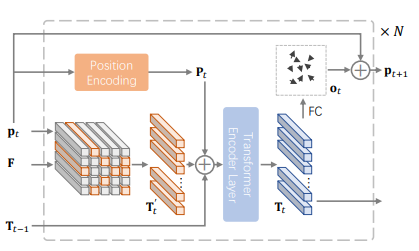
\includegraphics[scale = 0.7]{3}
\end{figure}
the feature map(F $\in \mathcal{R}^{C\times H\times W}$) extracted by the feature extractor module.Giving the sampling location $p_t\in \mathcal{R}^{2\times (n\times n)}$(the sampling points at the iteration t),where ($n\times n$) indicates the number of samples over one image and N is the total iterative number in the progressive sampling module.

For the first iteration, we  initialize the $p1$ to be the regularly-spaced locations.Concretely, the i-th location $p^i_1$(1 is the first iteration) is given by
$$\pi_i^y = \lfloor i/n\rfloor$$
$$\pi_i^x = i - \pi_i^y \times n$$
$$s_h = H/n$$
$$s_w = W/n$$
$$p_1^i = [\pi_i^ys_h + s_h/2,\pi_i^xs_w + s_w/2]$$
where $\pi_i^y$and $\pi_i^x$ map the location index i to the row index and the column one respectively.

Initial tokens are then sampled over the input feature map at the sampled locations as follows:
$$T'_t = F(p_t), t\in {1,...,N}$$
$T'_t\in \mathcal{R}^{C\times(n\times n)}$ are tokens sampled from F at the interation i.As elements of $p_t$ are fractional, the sampling is implemented via the bilinear interpolation operation.

$$P_t = W_tp_t$$
$$X_t = T'_x\oplus P_t \oplus T_{t-1}$$
$$T_t = Transformer(X_t), t\in {1,...,N}$$
$P_t\in \mathcal{R}^{C\times (n\times n)}$is the position embedding at the iteration t.$T'_t\in \mathcal{R}^{C\times (n\times n)}$is tokens sampled from F at the iteration t.$T_t\in \mathcal{R}^{C\times (n\times n)}$is tokens predicted by the progressive sampling module at the iteration t.$W_t\in \mathcal{R}^{C\times 2}$ is the linear transformation that projects the sampled location $p_t$ to the positional encoding matrix $P_t$ of size $C\times(n\times n)$,all iterations share the same $W_t$.Transformer(·) is the mulit-head self-attention based transformer encoder layer.
$$o_t = M_tT_t,t\in {1,...,N-1}$$
$M_t\in \mathcal{R}^{2\times C}$is the learnable linear transformation for predicting the sampling offset matrix.
\subsubsection{Overall Archtecture}

The architecture of the PS-ViT consists of four main components: 1) a feature extractor module to predict dense tokens; 2) a progressive sampling module to sample discriminative locations; 3) a vision
transformer module that follows the similar configuration of ViT and DeiT; 4) a classification module.

The feature extractor module aims at extracting the dense feature map F, where the progressive sampling module can simple tokens Tt. Each pixel of the dense feature map F can be treated as a token associated with a patch of the image.

\begin{figure}[h]
	\centering
	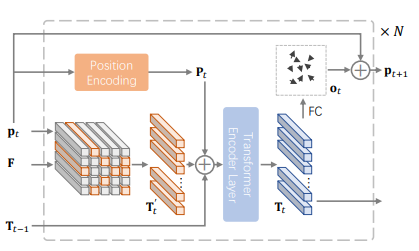
\includegraphics[scale = 0.7]{3}
\end{figure}
Given an input image, its feature map F is first extracted by the feature extractor module. Tokens $T_i$ are then sampled progressively and iteratively at adaptive locations $p_i$ over F in the progressive sampling module. The final output tokens $T_N$ of the progressive sampling module are padded with the classification token Tcls and further fed into the vision transformer module to refine $T_cls$, which is finally classified in the classification module.

We employ the convolutional stem and the first two residual blocks in the first stage of the ResNet50 as our feature extractor module.

We pad an extra token named by the classification token $T_{cls} \in \mathcal{R}^{C\times 1}$to the output tokens $T_N$ of the last iteration in the progressive sampling module, and feed them into the vision transformer module.And the output is $\mathcal{R}^{C\times (n\times n +1)}$

The vision transformer module follows the architecture adopted in ViT and DeiT.

The classification token refined through the vision transformer module is finally used to predict the image classes.
\subsubsection{Transformer Encoder Layer}
The transformer encoder layer serves as the basic building block for the progressive sampling module and the vision transformer module. Each transformer encoder layer has a multi-head self-attention and a feed-forward unit.

\section{PP-LCNet: A Lightweight CPU Convolutional Neural Network}

\subsection{Abstract}

This paper lists technologies which can improve network accuracy while the latency is almost constant. With these improvements, the accuracy of PP-LCNet can greatly surpass the previous network structure with the same inference time for classification

\subsection{Introduction}

As the model feature extraction capability increases and the number of model parameters and FLOPs get larger, it becomes difficult to achieve fast inference speed.

We consider the following three fundamental questions:
\noindent1.How to promote the network to learn stronger feature presentations without increasing latency.
\noindent2.What are the elements to improve the accuracy of lightweight models on CPU.
\noindent3.How to effectively combine different strategies for designing lightweight models on CPU.

We come up with several general rules for designing lightweight CNNs.

\subsection{Related Works}

Two types of methodologies to promote the capabilities of the models:
\noindent1.Manually-designed CNN Architecture.
\noindent2.Neural Architecture Search(NAS)

\subsubsection{Manually-designed Architecture}

VGG: Stacking blocks with the same dimension.

GoogLeNet: Inception block(including four parallel operation: 1 $\times$ 1 convolution, 3 $\times$ 3 convolution, 5 $\times$ 5 convolution and max pooling) which can make the convolution neural network light enough.

MobileNetV1: Depthwise and pointwise convolutions replace standard convolution.

MobileNetV2: Inverted block,which reduces the amount of parameters and FLOPs of the model.

ShuffleNetV1/V2: Exchange information through channel shuffle.

GhostNet: Ghost module, which can generate more feature maps with fewer parameters to improve the overall performance of the model.

\subsubsection{Neural Architecture Search}

MixNet: Hybridize depthwise converlations of different kernel size in one layer.

\subsection{Approach}

Here we have summarized some methods that can improve the performance of the model with little increase of inference time.

Concat or elementwise-add will not only slow down the inference speed of the model, but also will not improve the accuracy on a small model.

\begin{figure}[h]
	\centering
	
\includegraphics[scale = 0.5]{5}
\end{figure}
Stem Conv uses standard 3 $\times$ 3 convolution.DepthSepConv means depth-wise separable convolutions, DW means depth-wise convolution, PW means point-wise convolution, GAP means Global Average Pooling.
\subsubsection{Better Activation Function}

1.Sigmoid 2.ReLU 3.Swish activation funvtion 4.H-Swish

We replaced the activation function from ReLU to H-Swish.The performance has been grearly improved, while the inference time has hardly changed.

\subsubsection{SE Modules at Appropriate Position}

It does a good jib of weighting the network channels for better features,and its speed improvement version is also used in many lightweight networks.

The SE module increases the inference time,so that we cannot use it for the whole network.SE module is located at the end of the network,it can play a better role.So we just add the SE module to the blocks near the tail of the network.

The activation functions for the two layers of the SE module are ReLU and H-Sigmoid.

\subsubsection{Larger Convolution kernels}

The size of the convolution kernel often affects the final performance of the network.

However, mixing different sizes of convolutional kernels in the same layers of the network slows down the inference speed of the model, so we try to use only one size of convolution kernel in the single layer, and ensure that a large convolution kernel is used in the case of low latency and high accuracy.

We replace the 3 $\times$ 3 convolutional kernels with only the 5 $\times$ 5 convolutional kernels at the tail of the network would achieve the effect of replacing almost all layers of the network.
\subsubsection{Larger dimensional 1x1 conv layer after GPA}

When the output dimension of the network is small,in order to give the network a stronger fitting ability, we appended a 1280-dimensional size 1 $\times$ 1 conv(equivalent to FC layer) after the final GAP(Global Average Pooling) layer,which would allow for more storage of the model with little increase of inference time.

\subsection{Ablation Study}
\subsubsection{The impact of SE module in different positions}

\begin{figure}[h]
	\centering
	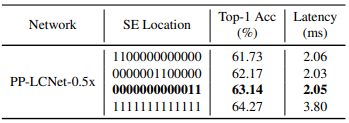
\includegraphics[scale = 0.5]{6}
\end{figure}
The table clearly shows that adding the last two blocks is more advantageous for almost the same inference time.
\subsubsection{The impact of large-kernel in different locations}

\begin{figure}[h]
	\centering
	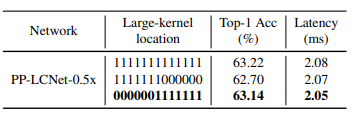
\includegraphics[scale = 0.5]{7}
\end{figure}
The table shows the positions added by the 5 $\times$ 5 depth-wise convolution.

1 means that the depth-wise convolution kernel in DepthSepConv is 5 $\times$ 5, and 0 means
that the depth-wise convolution kernel in DepthSepConv is 3 $\times$ 3.
\subsubsection{The impact of different techniques}

\begin{figure}[h]
	\centering
	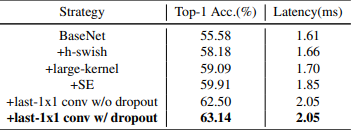
\includegraphics[scale = 0.5]{8}
\end{figure}
At the same time, perhaps because a relatively large matrix is involved here, the use of the dropout strategy can further improve the accuracy of the model.
\subsection{Conclution and Future Work}

The CNN used the approach shows stronger performance on a large number of vision tasks and has a better accuracy-speed balance.

In addition, this work reduces the search space of NAS and also offers the possibility of faster access to lightweight models for NAS.

In the future, we will also use NAS to obtain faster and stronger models.
\end{document}